\chapter{Sauerstoffinhalation mit Maske und Reservoir, Wechsel der Sauerstoffflasche}
\section{Inhalation mit Maske und Reservoir}
\begin{itemize}
    \item Reservoir muss gefüllt sein, bevor Maske aufgesetzt wird
    \item Bei Rettung aus vergifteter Atmosphäre / Tauchunfall wird in den meisten Fällen die CPAP Maske verwendet, sofern sie der Patient toleriert
\end{itemize}
\begin{figure}[H]
    \centering
    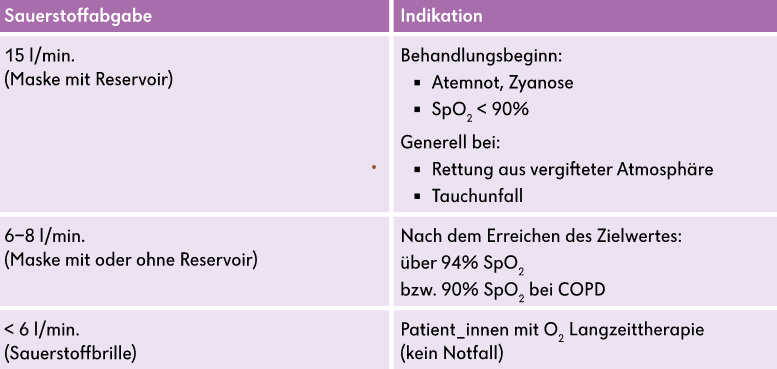
\includegraphics[width=\textwidth]{res/sauerstoff.png}
\end{figure}
\section{Wechsel der Sauerstoffflasche}
\begin{enumerate}
    \item Im Lager muss vermkert werden, welche Flaschen entnommen werden
    \item Bei der neuen Flasche soll (bevor der Druckminderer aufgesetzt wird) 1x kurz aufgedreht werden, damit Staub entfernt wird
    \item Danach kontrollieren, ob Flasche den erwüschten Druck enthält
\end{enumerate}